\documentclass{style}

\title{HSoE Hexacopter Project Documentation}
\author{\linkurl{https://github.com/nickgn12/hsoe-hexacopter-docs}}
\date{Last updated:\\ \today{}}

\begin{document}
\maketitle
\newpage
\tableofcontents
\newpage
\section{Battery}
\subsection{Charging}
\subsubsection{Connections}
Plug the charger into the mains using a three-pronged AC cable into the black AC port, or into the orange DC port if you have a DC cable with adapter.
To plug in the battery, first put the orange DC to positive/negative adapter on it, and then connect that to the positive and negative jacks on station 3 on the charger.
Do not plug the orange connector directly into the charging station, this is an input connection for the charger and will not charge the battery.
\subsubsection{Example Setup}
[Insert picture here]
\subsubsection{Charging Steps}
[Insert charging steps here]
\subsection{Connecting to Flight Controller}
Slide the battery into the slot underneath the flight controller so that the velcro on the battery lines up to the velcro on the frame and sticks to it.
Connect the orange connector on the battery to the orange connector attached to the frame.
Once connected to the flight controller, it should beep three times using the motors, followed by a one second delay, and then one final long beep.
\section{Flight Controller}
The hexacopter is currently using an \textit{ArduCopter} flight controller.
A \textit{PixHawk} was previously used, but was found to be defective.
It can still be found in the hexacopter project bag.
\subsection{Motors Connection}
\subsection{I2C Connection}
\subsection{Power Connection}
\subsection{Compass Connection}
\section{Remote Controller}
\subsection{Controls}
\begin{tabular}{ l l l }
  \textbf{Stick} & \textbf{Axis} & \textbf{Function} \\
  Left & Y & Throttle Up/Down \\
  Left & X & Yaw Left/Right \\
  Right & Y & Pitch Up/Down \\
  Right & X & Roll Left/Right
\end{tabular}
\subsection{Arming/Disarming}
[Find out how to arm the copter using the controller]
\section{Propellers}
\subsection{Sizes}
The propellers should be size [xyz].  The top three propellers all spin clockwise, and should be labelled SFP.  The bottom three propellers spin counter-clockwise and should be labelled SP.
\subsection{Attaching to Motors}
When placing the propellers onto the motors, the propellers should be placed first, divot side up.
It is then followed by the washer and then the nut.
To prevent the nuts from flying off during flight, Loctite or any similar adhesive should be applied to secure them to the screws.
\section{Telemetry}
The hexacopter can be connected to a computer to probe for debug info or to arm/disarm the craft. \\ \\
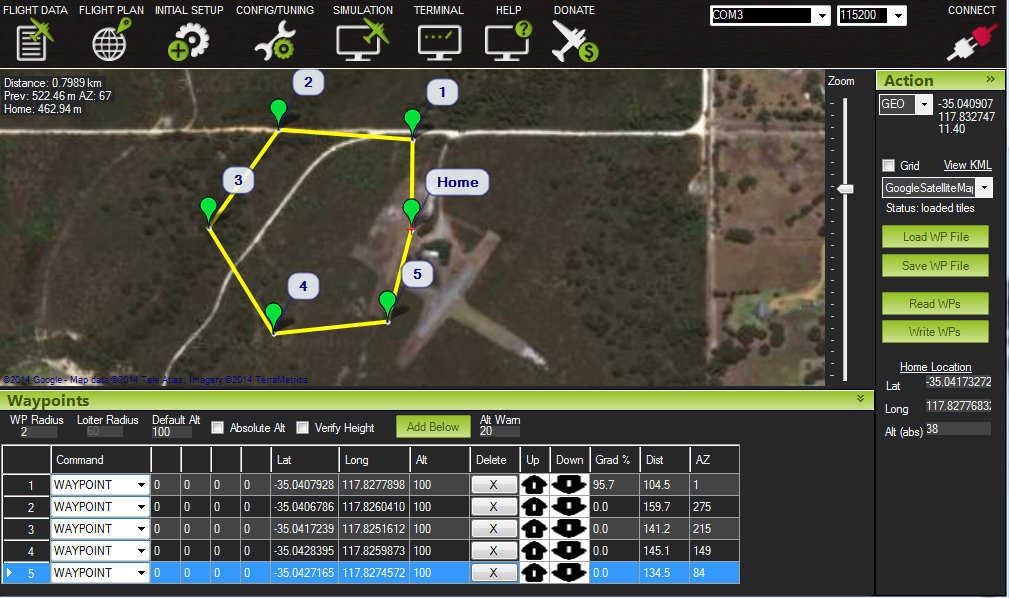
\includegraphics[scale=0.5]{mission_planner.jpg} \\
(example screenshot of APM Planner)
\subsection{Download}
\link{http://firmware.us.ardupilot.org/Tools/APMPlanner/}{APM Planner} - (MacOS, Linux, Windows) \\
\link{http://ardupilot.org/planner/docs/common-install-mission-planner.html}{Mission Planner} - (Windows only)
\subsection{Direct Connection}
To direct connectly to the craft, plug a micro-usb connector into the \textit{ArduCopter} flight controller, and the other end in an empty USB connector on a computer.
Start up either APM Planner or Mission Planner and hit the connect button.
Depending on your operating system of choice, the flight controller will show up as different things:
\newline
\newline
\begin{tabular}{ l l }
  Windows & \texttt{COMx} \\
  OS/X & \texttt{tty.usbSerialXXX} \\
  Linux & \texttt{ttyUSBx}
\end{tabular}
\subsection{Radio}
I couldn't get this working yet :/
\pagebreak
\section{Todo}
\begin{itemize}
\item 1.1.2 Charging connections example setup
\item 1.1.3 Charging steps
\item 2 Figure out how to arm w/ controller
\item 4.3 Figure out how to get the radio telemetry working
\item Get lots of pictures
\end{itemize}
\end{document}
